% LaTeX file for Chapter 02



\begin{knitrout}
\definecolor{shadecolor}{rgb}{0.969, 0.969, 0.969}\color{fgcolor}\begin{kframe}
\begin{alltt}
\hlkwd{library}\hlstd{(knitr)}
\hlstd{opts_chunk}\hlopt{$}\hlkwd{set}\hlstd{(}\hlkwc{fig.path}\hlstd{=}\hlstr{'figure/ch02_fig'}\hlstd{,}
               \hlkwc{echo}\hlstd{=}\hlnum{TRUE}\hlstd{,} \hlkwc{message}\hlstd{=}\hlnum{FALSE}\hlstd{,}
               \hlkwc{fig.width}\hlstd{=}\hlnum{9}\hlstd{,} \hlkwc{fig.height}\hlstd{=}\hlnum{3.5}\hlstd{,}
               \hlkwc{out.width}\hlstd{=}\hlstr{'\textbackslash{}\textbackslash{}textwidth-3cm'}\hlstd{,}
               \hlkwc{message}\hlstd{=}\hlnum{FALSE}\hlstd{,} \hlkwc{fig.align}\hlstd{=}\hlstr{'center'}\hlstd{,}
               \hlkwc{background}\hlstd{=}\hlstr{"gray98"}\hlstd{,} \hlkwc{tidy}\hlstd{=}\hlnum{FALSE}\hlstd{,} \hlcom{#tidy.opts=list(width.cutoff=60),}
               \hlkwc{cache}\hlstd{=}\hlnum{TRUE}
\hlstd{)}
\hlkwd{options}\hlstd{(}\hlkwc{width}\hlstd{=}\hlnum{74}\hlstd{)}
\end{alltt}
\end{kframe}
\end{knitrout}





\chapter{The Cochrane Dataset} 


\subsection{Structure and Content}
The dataset consists of 5006 reviews from the Cochrane Library. The sum of distinct studies in the single reviews is 62278 (some of them might being shared among reviews). In figure \ref{studies.per.review}, the empirical distribution of the number of distinct studies per review is depicted. It can be seen that while almost 400 reviews consist of one study only, there are almost 500 with equal or more than 30 distinct studies. 

\label{studies.per.review}
\begin{knitrout}
\definecolor{shadecolor}{rgb}{0.98, 0.98, 0.98}\color{fgcolor}

{\centering 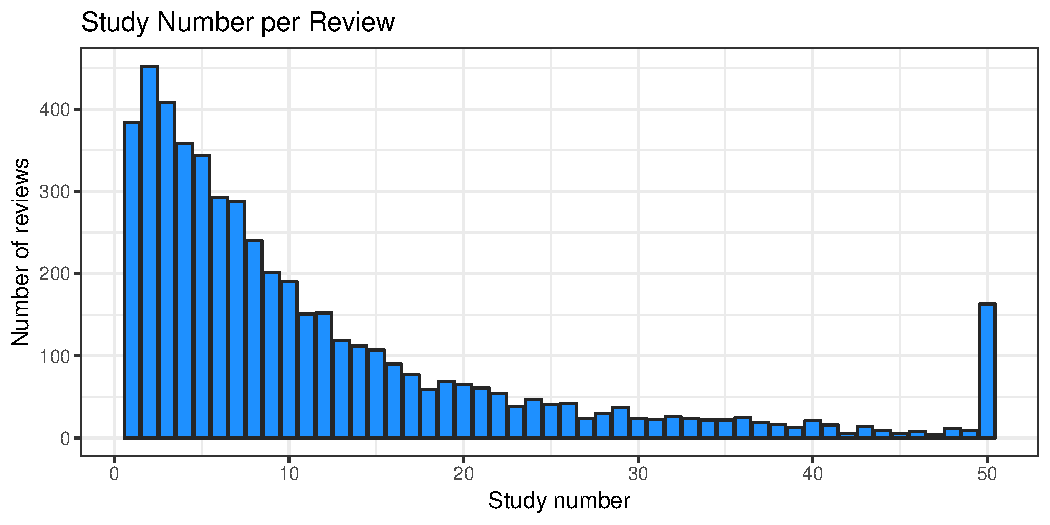
\includegraphics[width=\textwidth-3cm]{figure/ch02_figunnamed-chunk-3-1} 

}



\end{knitrout}

% (DOI: 10.1002/14651858.CD000033.pub2). 
Depending on the scope of the research question, it comprises a range of research subjects. As an example, consider a review about barbiturate effect on head injuries 
There are different drugs of the barbiturate class, that can again be compared to placebo or other drugs. Therefore, the studies in a review can again be distinguished by their research subject. Again, figure \ref{subjects.per.review} provides an illustration of the distribution of the number of different research subjects per review.

\label{subjects.per.review}
\begin{knitrout}
\definecolor{shadecolor}{rgb}{0.98, 0.98, 0.98}\color{fgcolor}

{\centering 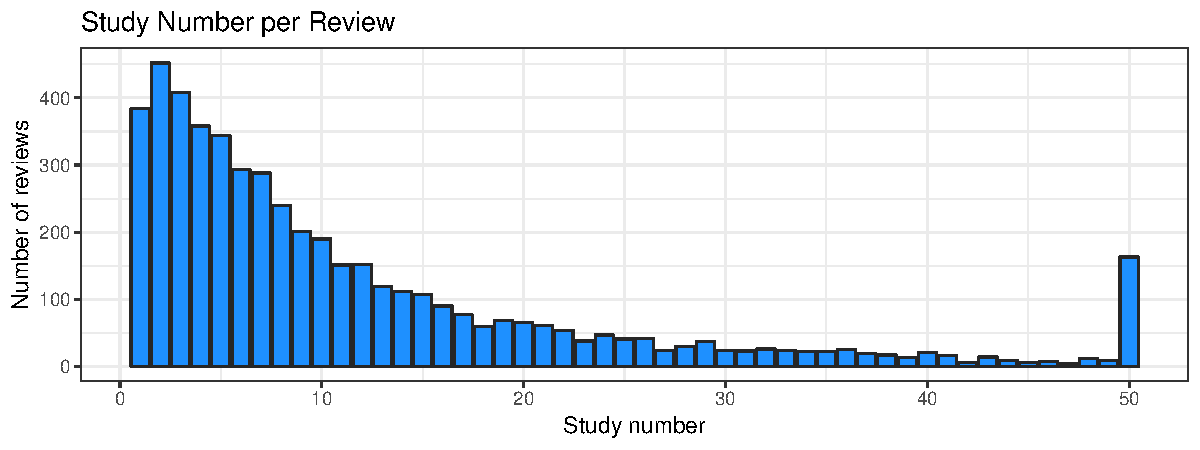
\includegraphics[width=\textwidth-3cm]{figure/ch02_figunnamed-chunk-4-1} 

}



\end{knitrout}

Despite that studies within a review cover the same research subject, they could still be different with respect to their outcome. For example, in the case of the barbiturate and head injury review, different measurements of mortality (e.g. after 6 or 12 months) could be considered. This is of particular importance if one is to compare the results directly. Considering this, one might want to look at the distribution of number of different outcomes within a review (given that the research subject is the same). If one sums up the number of different outcomes given that they share the research subject, the empirical distribution of the sums can be seen in figure \ref{outcomes.per.review}. It is necessary to consider the research subject, because it can be that the outcome is the same (mortality after ..) but not the research subject (other barbiturate). One can see that the heterogeneity considering research subjects and outcomes between reviews is considerably large. Almost 500 reviews have more than 50 different experimental settings, i.e. different research subjects and outcome measures. The mean number of different outcome measures is 21.67 and the median 13 

\label{outcomes.per.review}
\begin{knitrout}
\definecolor{shadecolor}{rgb}{0.98, 0.98, 0.98}\color{fgcolor}

{\centering 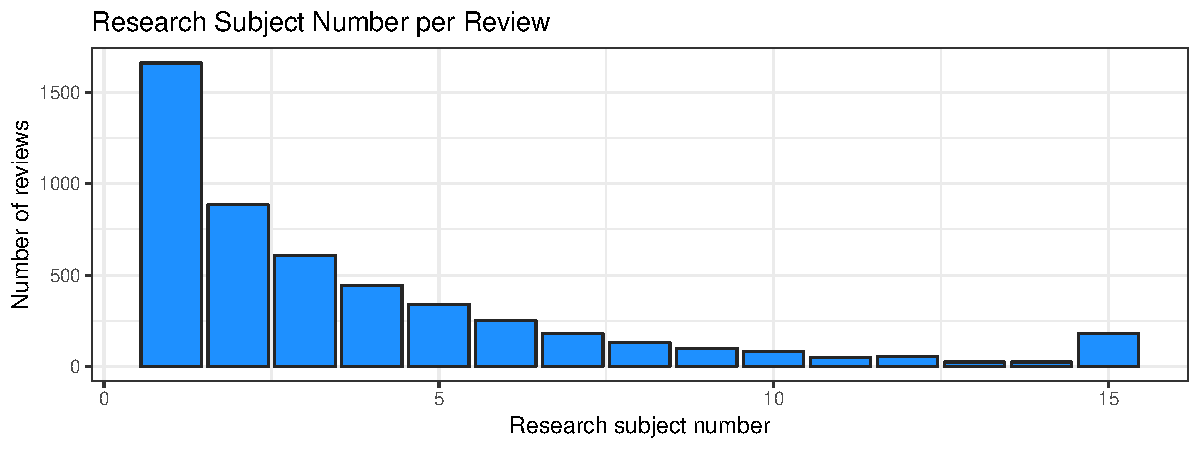
\includegraphics[width=\textwidth-3cm]{figure/ch02_figunnamed-chunk-5-1} 

}



\end{knitrout}























































% Maybe it is the methods section. Here however, we give a couple hints.
% Note that you can wisely use \rr{preamble}-chunks. Minimal, is likely: 
% 
% \bigskip
% 
% \hrule
% <<echo=TRUE>>=
% library(knitr) 
% opts_chunk$set( 
%     fig.path='figure/ch02_fig',    
%     self.contained=FALSE,
%     cache=TRUE
% ) 
% @
% \hrule
% 
% \bigskip
% 
% Defining figure options is very helpful:
% 
%  
% \bigskip
% 
% 
% \hrule
% <<echo=TRUE>>=
% library(knitr)
% opts_chunk$set(fig.path='figure/ch02_fig',
%                echo=TRUE, message=FALSE,
%                fig.width=8, fig.height=2.5,  
%                out.width='\\textwidth-3cm',
%                message=FALSE, fig.align='center',
%                background="gray98", tidy=FALSE, #tidy.opts=list(width.cutoff=60),
%                cache=TRUE
% ) 
% options(width=74)
% @ 
% \hrule
% 
% \bigskip 
% 
% Notice how in Figure~\ref{f02:1} everything is properly scaled.   
% 
% \begin{figure}
% <<echo=FALSE>>=
% par(mai=c(.8,.8,.1,.1)) 
% set.seed(12)
% plot( runif(30), type='l')
% @   
%   \caption{Test figure to illustrate figure options used by knitr.}
%   \label{f02:1}
% \end{figure}
